\section{ASZ Optimization Strategies}
\label{sec:optimization-strategies}

In this section, we present ASZ's new predictors and per-round choices of prediction axis and QB serialization order, together with methods for tuning them efficiently:
\begin{itemize}
\item Sections~\ref{sec:configuration-space:predictors}--\ref{sec:configuration-space:reference-count} design and evaluate the \emph{variable-coefficient predictors}.
\item Section~\ref{sec:configuration-space:serialization} creates and evaluates per-round \emph{QB serialization orders}.
\item Sections~\ref{sec:configuration-space:coefficient-selection} and~\ref{sec:configuration-space:coefficient-evaluation} develop \emph{fast coefficient selection} through a rate--distortion proxy and reusable statistics.
\item Section~\ref{sec:configuration-space:reverse-greedy} uses \emph{reverse-greedy search} to generate the configuration plan without exhaustive enumeration.
\end{itemize}
\subsection{Candidate Prediction Stencils}
\label{sec:configuration-space:predictors}

ASZ constructs three variable-coefficient predictors from the candidate prediction stencils: 1D4R, 2D4R, and 1D6R. In these abbreviations, 1D and 2D indicate that the references are drawn from one and two coordinate axes, respectively, while 4R and 6R indicate the use of four and six reference points.

We first generalize SZ3's cubic interpolation to the following 1D4R form, using the local coordinates illustrated in Fig.~\ref{fig:background:stencils}(b):
\begin{equation}
\label{eq:configuration-space:1d4r-prediction}
p(t)=(\tfrac14+t)(\hat x_{-h}+\hat x_h)+(\tfrac14-t)(\hat x_{-3h}+\hat x_{3h}).
\end{equation}
Like the fixed formulas used by SZ3 and QoZ, this predictor assigns equal coefficients to references symmetric about the target and constrains the four coefficients to sum to one, thereby preserving exact prediction of constant-valued data. The predictor recovers SZ3's cubic interpolation at $t=5/16$, reduces to SZ3's linear interpolation at $t=1/4$, and becomes four-point equal-weight averaging at $t=0$.

In addition, we consider variable-coefficient 2D4R and 1D6R predictors. The 2D4R predictor follows QoZ's two-dimensional linear prediction, which combines linear predictions along two axes. Using the local coordinates illustrated in Fig.~\ref{fig:background:stencils}(d), we write
\begin{equation}
\label{eq:configuration-space:2d4r-prediction}
p(t)=(\tfrac14+t)(\hat x_{-h_0,0}+\hat x_{h_0,0})+(\tfrac14-t)(\hat x_{0,-h_1}+\hat x_{0,h_1}).
\end{equation}
Unlike QoZ's two-pass cubic predictor, ASZ's 1D6R predictor uses three symmetric reference pairs at offsets $h$, $3h$, and $5h$, all reconstructed before the current round. Its targets therefore remain independent within a round, allowing ASZ to apply the predictor in one pass and avoid the overhead of a second prediction pass. We parameterize the per-reference weights as
\begin{equation}
\label{eq:configuration-space:1d6r-prediction}
\begin{aligned}
p(a,b)&=(\tfrac12-a-b)(\hat x_{-h}+\hat x_h)\\
&\quad+b(\hat x_{-3h}+\hat x_{3h})\\
&\quad+a(\hat x_{-5h}+\hat x_{5h}).
\end{aligned}
\end{equation}
This predictor recovers fixed six-point quintic interpolation at $a=3/256$ and $b=-25/256$.

\begin{figure}[htb]
\centering
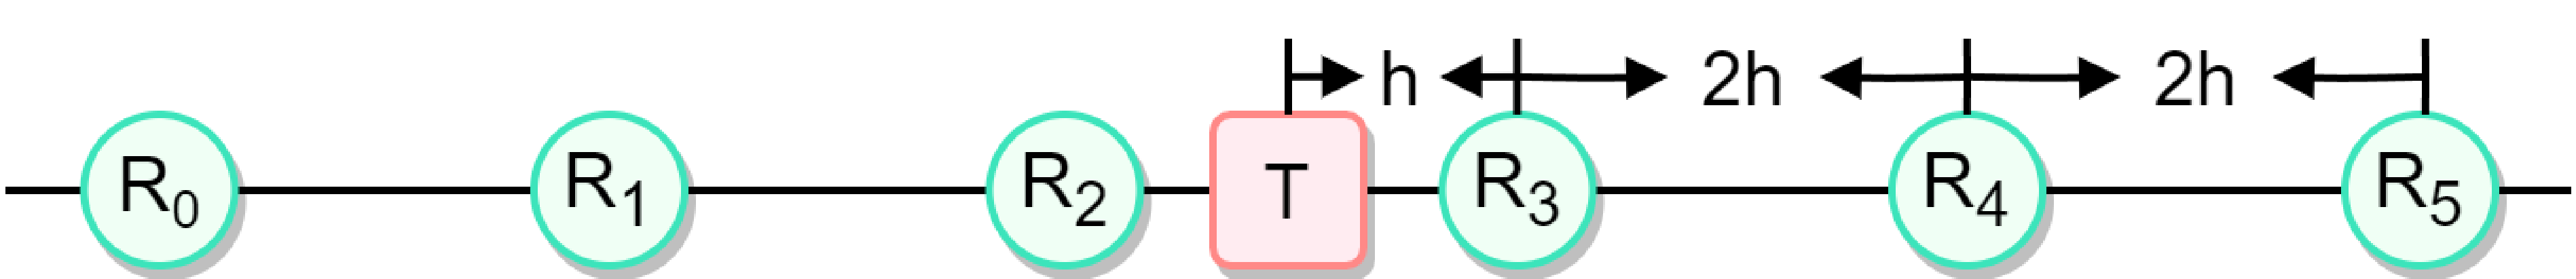
\includegraphics[width=\columnwidth]{revised-fig/1d6r-prediction-stencil.pdf}
\caption{Reference layout of the 1D6R prediction stencil. The six references lie at offsets $\pm h$, $\pm3h$, and $\pm5h$ from target $T$ and are reconstructed before the current round. Targets within the round therefore remain independent and can be predicted in a single pass, reducing prediction overhead.}
\label{fig:configuration-space:1d6r-stencil}
\end{figure}

\subsection{One- versus Two-Dimensional Prediction}
\label{sec:configuration-space:dimensionality}

We compare the compression performance of 1D4R and 2D4R to determine which prediction stencil to retain. Figure~\ref{fig:configuration-space:1d4r-vs-2d4r} reports their rate--distortion curves on three datasets. We evaluate the three individual prediction axes for 1D4R and the three axis pairs for 2D4R, selecting the best coefficient and QB serialization order for each. We find that 1D4R provides a better overall rate--distortion trade-off than 2D4R and therefore exclude 2D4R from the remaining configuration space.

\begin{figure}[htb]
\centering
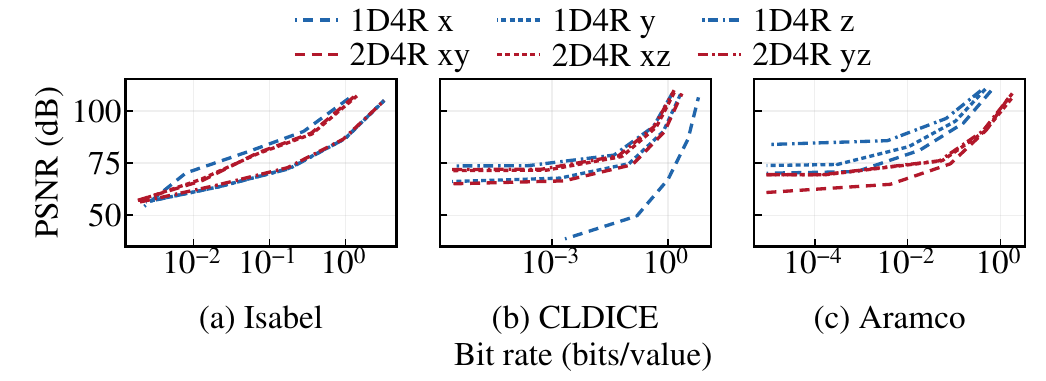
\includegraphics[width=\columnwidth]{revised-fig/raster300/iv-1d4r-vs-2d4r-legacy-middle.png}
\caption{Rate--distortion comparison of 1D4R and 2D4R. Each curve represents one prediction axis for 1D4R or one pair of prediction axes for 2D4R after selecting the best coefficient and QB serialization order. We observe a better overall rate--distortion trade-off with 1D4R in all three cases.}
\label{fig:configuration-space:1d4r-vs-2d4r}
\end{figure}

One possible explanation follows from how the two predictors correct their underlying linear predictions. In 1D4R, outer references provide a higher-order correction to inner two-point linear interpolation. The coefficient controls its strength and disables it at $t=1/4$. This correction may remain consistently useful or useless within a local region. By contrast, 2D4R is mathematically equivalent to a weighted average of two linear predictions, one along each axis. Their errors may cancel at one target but not at a nearby target, limiting the spatial extent over which the same blending weights remain effective.

This comparison concerns variable-coefficient predictors. QoZ's multidimensional interpolation combines predefined per-axis linear or cubic formulas and adapts their directional blending weights. The ASZ predictors instead allow the reference coefficients along each axis to vary.

\subsection{Four- versus Six-Reference Prediction}
\label{sec:configuration-space:reference-count}

Figure~\ref{fig:configuration-space:1d4r-vs-1d6r} shows that 1D4R and 1D6R perform nearly identically in most cases, while 1D6R offers advantages on some data files. Each predictor is evaluated along three prediction axes and therefore contributes three curves to each plot.

\begin{figure}[htb]
\centering
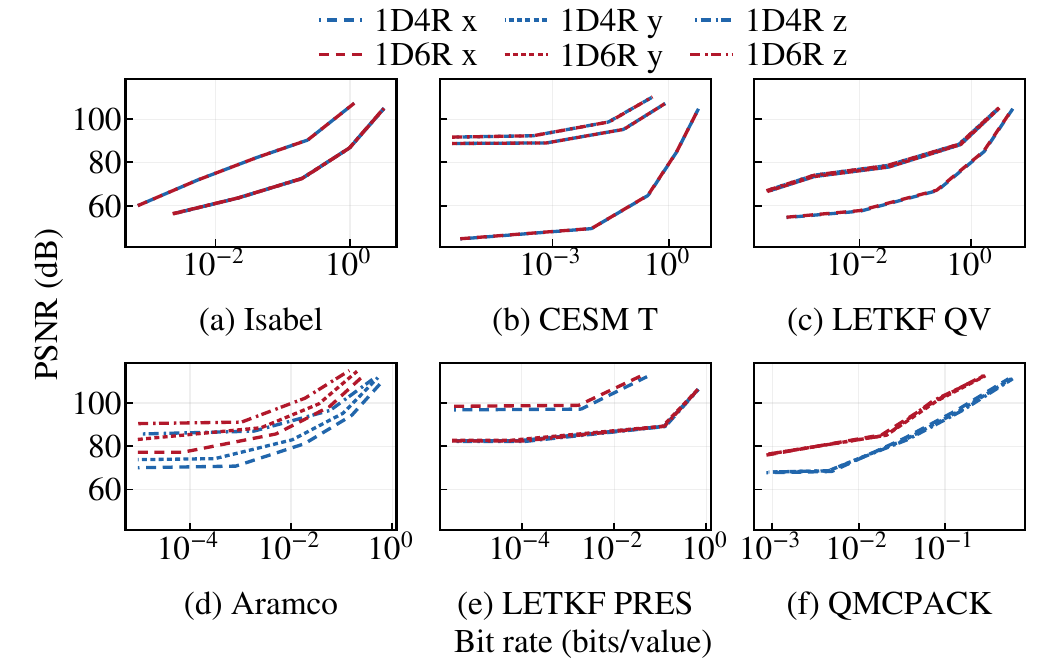
\includegraphics[width=\columnwidth]{revised-fig/raster300/iv-1d4r-vs-1d6r-legacy-middle.png}
\caption{Rate--distortion comparison of 1D4R and 1D6R. Each predictor contributes three curves, one per axis. The two predictors perform nearly identically in (a)--(c), whereas 1D6R offers advantages in (d)--(f).}
\label{fig:configuration-space:1d4r-vs-1d6r}
\end{figure}

Figure~\ref{fig:configuration-space:1d6r-coefficients} further compares 1D6R under 42 fixed coefficient pairs. Each curve retains one coefficient pair after selecting its best prediction axis at each error bound.

\begin{figure}[htb]
\centering
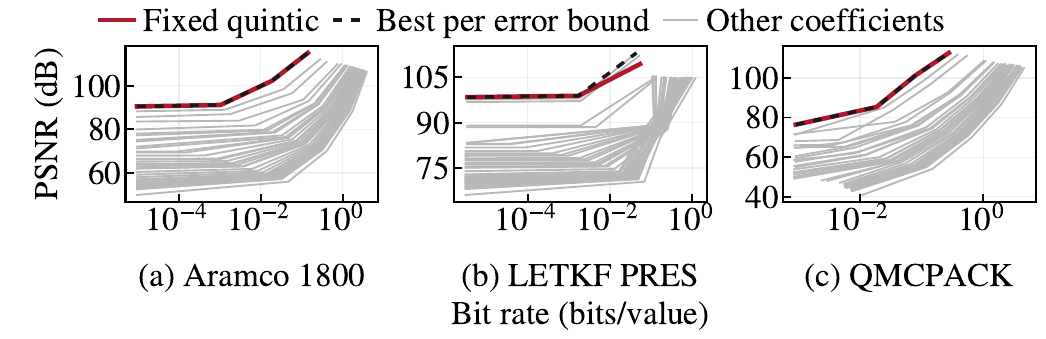
\includegraphics[width=\columnwidth]{revised-fig/raster300/iv-1d6r-coefficients.png}
\caption{Rate--distortion curves for 42 fixed 1D6R coefficient pairs. Fixed quintic interpolation is among the strongest settings overall.}
\label{fig:configuration-space:1d6r-coefficients}
\end{figure}

Coefficient tuning offers less benefit for 1D6R than for 1D4R. In both predictors, tuning controls a higher-order correction to a lower-order interpolation formula. The 1D4R parameter can continuously weaken the cubic correction and disable it entirely, recovering two-point linear interpolation when the outer references are unreliable. In fixed-quintic 1D6R, each of the two additional outermost references has a weight of only about $1.2\%$ and provides a small correction to cubic interpolation. Small coefficient changes have little effect, while large changes remove its ability to cancel the higher-order error left by cubic interpolation. Consistent with this narrow useful range, Fig.~\ref{fig:configuration-space:1d6r-coefficients} shows little gain from tuning the two 1D6R coefficients. ASZ therefore tunes 1D4R, retains fixed-quintic coefficients for 1D6R, and chooses between the two predictors using sampled mean squared prediction error.

% TODO: 最佳系数来自指定的有限网格，而非所有实数系数的全局最优。正式报告各prediction stencil的网格范围和步长。
% 第一组实测结果：results/predictor-family-legacy-middle-21244405。单轮、固定原始参考值、stencil-specific目标集合；机制段落是可能的解释，不是1D4R必然胜出的理论证明。
% 第二组实验：Fig. 3为单栏两行三列。上排Isabel Pf24、CESM T t31、LETKF QV (log10)，下排Aramco 1800、LETKF PRES、QMCPACK orbital 0。使用results/predictor-family-4r6r-middle-21250842-recovered、results/predictor-family-4r6r-supplement-21274865-recovered及results/predictor-family-4r6r-qmcpack-orbital0-20261011。CLDICE原始测量仍保留，未计入当前六图；上排三例接近重合，Aramco与QMCPACK明显受益、PRES较温和。QMCPACK依据已有原始参考MSE选择为收益案例，因此此图不能用于估计总体收益出现频率。
% 固定系数比较：results/1d6r-coefficients-three-20261011，每个数据42个系数各选5个方向/QB顺序最优点。QMCPACK为新增完整穷举，其他数据复用原始CSV。只有PRES的0.1端点局部参考完全重合且各轴码率不等，显式--expand-flat-reference扩至0.1与0.001的平均RD点，其他评分参考不变；具体端点及原CSV哈希保存在CSV/JSON。图4红线为固定五次系数，黑虚线为各误差界独立选择系数的最优点连线，并非另一个固定系数或插值后的包络。QMCPACK的5个误差界均选择固定五次系数，按三个方向分别选择时15个点也均为固定五次系数。
% TODO: PRES在1e-5下过渡系数(247/1536,379/1536)、x方向、xx2优于固定五次系数：BR=0.043723358585859、PSNR=113.0988287234236；固定五次最佳BR=0.053443181818182、PSNR=109.41677733253238，甚至被1D4R的BR=0.051559848484848、PSNR=112.171002012328898压倒。因此结论为固定五次系数总体表现较好，不能写“总是最优”；仍需量化固定系数的完整压缩损失。
% TODO: results/predictor-family-paper-refined与revised-fig/predictor-family-refined为共享目标、原始参考值固定的采样单轮诊断，不能当作完整ASZ压缩器结果。历史完整压缩器选择器验证的来源为results/predictor_family_rd_extremes_*.csv，仍需扩展数据和误差界检验泛化。
% 第二组候选使用transition模式的42组有理数参数，覆盖全部13组1D4R；shared1d模式统一四点和六点预测的目标位置。结论依据实际RD结果，不能由ASZ选择记录代替。

\subsection{Quantization-Bin Serialization Order}
\label{sec:configuration-space:serialization}

QB serialization order specifies the order in which quantized residual symbols are passed to lossless compression. For a fixed QB multiset, the Huffman code lengths and total Huffman size depend on symbol frequencies rather than symbol order. Reordering instead changes the sequence of Huffman codewords and hence the byte-level patterns presented to the subsequent Zstd stage. QB serialization-order tuning therefore primarily targets Zstd compression.

SZ3 and QoZ serialize QBs in generation order, which naturally keeps the QBs produced in the same prediction round together. These QBs share a stencil and reference spacing, and therefore tend to have similar prediction accuracy and symbol distributions. This round-wise grouping gives the lossless stage a stream with locally consistent statistics. ASZ retains this organization and never interleaves QBs from different rounds.

ASZ makes the QB serialization order within each round configurable. Weighted-sum prediction can leave residual spatial correlation along any coordinate axis, and the prediction axis need not have the strongest residual correlation. Equal QBs may therefore form runs along another axis. Making that axis the fastest-varying dimension places these symbols consecutively in the stream and exposes the run to Zstd. To create this configuration dimension, ASZ stores the QBs of a round as a three-dimensional tensor and exposes three linearizations, one for each possible fastest-varying dimension. The relative order of the two slower dimensions has little effect on Zstd, so ASZ need not expose all six axis permutations.

All three choices preserve the QBs, their histogram, and reconstruction, so they have identical $H_1$ and PSNR. ASZ therefore compares them through sample-based trial compression.

Figure~\ref{fig:configuration-space:qb-order} summarizes exhaustive trials for the finest prediction round on three data files. For each error bound and QB serialization order, the plotted point is the best measured BR--PSNR candidate among three prediction axes and eleven coefficients $t\in\{2/32,\ldots,12/32\}$.

\begin{figure}[htb]
\centering
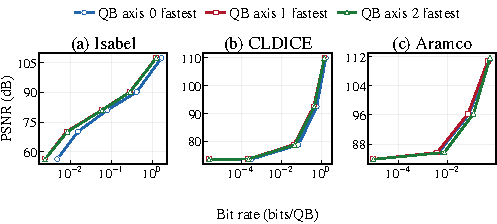
\includegraphics[width=\columnwidth]{revised-fig/qb-order-rd.pdf}
\caption{Rate--distortion comparison of QB serialization orders after independently selecting the best prediction axis and coefficient for each order. Labels 0, 1, and 2 identify the fastest-varying dimension of the serialized QB tensor.}
\label{fig:configuration-space:qb-order}
\end{figure}

Among the 15 data-file--error-bound cases, the order with dimension 1 varying fastest is uniquely best in ten cases and the order with dimension 2 varying fastest in two, while all three orders tie in the remaining three. The preferred order therefore varies across data and operating points, which motivates retaining QB serialization order as a round-wise configuration choice.

\subsection{Proxy-Based Coefficient Selection}
\label{sec:configuration-space:coefficient-selection}

After predictor pruning, coefficient tuning applies only to 1D4R and its scalar coefficient $t$. ASZ ranks candidates with an $H_1$--PSNR proxy, which replaces compressed bit rate with the first-order entropy $H_1$ of the quantization bins (QBs). BR--PSNR provides the reference ranking used to validate this proxy.

At a fixed error bound, each coefficient candidate is a point in the BR--PSNR plane, where better performance lies toward the upper left. The score must account for simultaneous changes in bit rate and PSNR. As illustrated in Fig.~\ref{fig:configuration-space:rd-score}, we project each candidate onto the normal of the local reference tangent that points toward the upper left. A candidate projected farther along this normal receives a larger score.

\begin{figure}[htb]
\centering
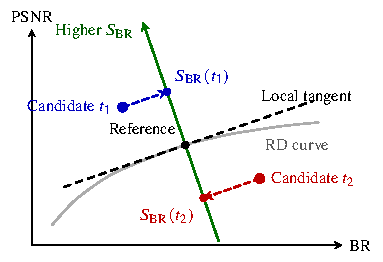
\includegraphics[width=0.95\columnwidth]{revised-fig/rd-score-geometry.pdf}
\caption{Geometric interpretation of the BR--PSNR score. Dashed lines project candidates parallel to the local tangent onto its normal, which serves as the score axis.}
\label{fig:configuration-space:rd-score}
\end{figure}

For a fixed dataset, error bound, prediction stencil, and prediction axis, the BR--PSNR score of coefficient $t$, computed using its measured Huffman--Zstd QB-stream bit rate, is
\begin{equation}
\label{eq:configuration-space:br-psnr-score}
S_{\mathrm{BR}}(t)=\frac{\mathrm{PSNR}(t)-m_{\mathrm{BR}}\mathrm{BR}(t)}{\sqrt{1+m_{\mathrm{BR}}^2}},
\end{equation}
where $m_{\mathrm{BR}}$ ideally denotes the local slope of the BR--PSNR curve at the operating point. Because this derivative is not directly available, ASZ approximates it by the finite difference between two neighboring error bounds. A larger score indicates greater displacement toward higher PSNR and lower BR and is therefore preferred.

Exact evaluation of $S_{\mathrm{BR}}(t)$ performs Huffman--Zstd compression on the QB stream produced by every candidate $t$. ASZ replaces BR--PSNR with $H_1$--PSNR for candidate selection. Let $p_q(t)$ be the fraction of targets assigned to QB $q$ under coefficient $t$. Its first-order entropy is
\begin{equation}
\label{eq:configuration-space:h1}
H_1(t)=-\sum_{q:p_q(t)>0}p_q(t)\log_2p_q(t),
\end{equation}
measured in bits per QB. Analogous to Eq.~\eqref{eq:configuration-space:br-psnr-score}, we define the $H_1$--PSNR score as
\begin{equation}
\label{eq:configuration-space:h1-psnr-score}
S_{H_1}(t)=\frac{\mathrm{PSNR}(t)-m_{H_1}H_1(t)}{\sqrt{1+m_{H_1}^2}},
\end{equation}
where $m_{H_1}$ is the corresponding local slope, estimated in the same way as $m_{\mathrm{BR}}$.

$H_1$ depends only on QB frequencies and therefore requires neither lossless compression nor an ordered QB stream. It omits QB serialization order and the sequence patterns exploited by Zstd, so it can either overestimate or underestimate BR. The validation below shows that $H_1$--PSNR usually selects the same coefficient as BR--PSNR. ASZ selects the candidate with the largest $S_{H_1}$.

Jin et al.~\cite{jin2022improving} use entropy and modeled PSNR to estimate absolute rate--quality curves. ASZ uses $H_1$ only as a relative rate proxy, derives coefficient-specific PSNR from post-quantization residual distributions, and combines the two through $S_{H_1}$ to rank coefficients at a fixed error bound, prediction stencil, and prediction axis. Section~\ref{sec:configuration-space:coefficient-evaluation} shows how one coefficient-independent joint distribution evaluates all candidates.

\begin{figure}[htb]
\centering
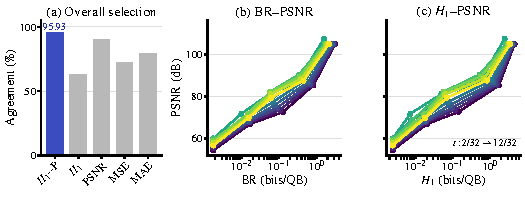
\includegraphics[width=\columnwidth]{revised-fig/coefficient-proxy-validation.pdf}
\caption{Coefficient-selection proxy validation. (a) $H_1$--PSNR achieves the highest overall agreement with BR--PSNR among the proxy criteria, at 95.93\%. (b)--(c) Sets of BR--PSNR and $H_1$--PSNR curves for Isabel Pf24 along the first coordinate axis. Each color denotes one coefficient $t\in\{2/32,\ldots,12/32\}$, and each curve contains the five relative error bounds from $10^{-1}$ to $10^{-5}$.}
\label{fig:configuration-space:global-coefficient-selection}
\end{figure}

Figure~\ref{fig:configuration-space:global-coefficient-selection} reports how often each criterion selects the same file-wide coefficient as BR--PSNR, which uses measured compressed rate and reconstruction quality. For each data file, error bound, and 1D4R prediction axis, we evaluate the eleven candidates $t\in\{2/32,\ldots,12/32\}$. The candidate with the largest $S_{\mathrm{BR}}$ is the reference choice. Each proxy independently selects its best candidate, and an agreement means that the two choices coincide.

Panels (b) and (c) provide a representative visual comparison of the two sets of curves. Although $H_1$ is not a numerical estimate of BR, replacing BR with $H_1$ largely preserves the relative arrangement of the coefficient curves. $H_1$--PSNR agrees with BR--PSNR in 95.93\% of the tests. The other criteria are less accurate because each omits either coding cost or reconstruction quality.

\subsection{Reusable Coefficient Evaluation}
\label{sec:configuration-space:coefficient-evaluation}

ASZ evaluates $H_1(t)$ and PSNR$(t)$ for many coefficient candidates from the prediction-error distribution $f_t(e)$. Let $\Delta$ be the QB interval, $R$ the data range, and $\mathcal{Q}_q=[(q-\tfrac12)\Delta,(q+\tfrac12)\Delta)$ the errors mapped to QB $q$. The QB probability and the post-quantization mean squared error are
\begin{equation}
\label{eq:configuration-space:distribution-metrics}
\begin{aligned}
p_q(t)&=\int_{\mathcal{Q}_q}f_t(e)\,de,\\
D(t)&=\sum_q\int_{\mathcal{Q}_q}(e-q\Delta)^2f_t(e)\,de.
\end{aligned}
\end{equation}
The probabilities $p_q(t)$ yield $H_1(t)$ through Eq.~\eqref{eq:configuration-space:h1}, while $D(t)$ yields $\operatorname{PSNR}(t)=10\log_{10}(R^2/D(t))$. Coefficient evaluation therefore requires the error distribution rather than the locations or order of individual targets.

For 1D4R, the error distributions for all candidates can be obtained from one coefficient-independent joint distribution. For target $x_i$, define the outer and inner reference sums as $O_i=\hat x_{-3h}+\hat x_{3h}$ and $I_i=\hat x_{-h}+\hat x_h$, respectively. From Eq.~\eqref{eq:configuration-space:1d4r-prediction}, its prediction error is
\begin{equation}
\label{eq:configuration-space:affine-error}
e_i(t)=x_i-p_i(t)=A_i t+B_i,
\end{equation}
where $A_i=O_i-I_i$ and $B_i=x_i-(O_i+I_i)/4$. Both terms are independent of $t$. Thus, the joint distribution of $(A,B)$ determines $f_t(e)$ for every $t$.

ASZ samples $n$ targets, computes their $(A_i,B_i)$ pairs once, and quantizes the two values onto a fine two-dimensional grid. Let $(a_j,b_j)$ and $c_j$ denote the center and count of occupied grid cell $j$. For candidate $t$, each cell contributes the approximate error $\tilde e_j(t)=a_jt+b_j$. We quantize this error as
\begin{equation}
\label{eq:configuration-space:histogram-estimates}
\begin{aligned}
\tilde q_j(t)&=\operatorname{round}\!\left(\frac{\tilde e_j(t)}{\Delta}\right),&
\tilde d_j(t)&=\tilde e_j(t)-\Delta\tilde q_j(t),\\
\hat p_q(t)&=\frac1n\sum_{j:\tilde q_j(t)=q}c_j,&
\hat D(t)&=\frac1n\sum_jc_j\tilde d_j(t)^2.
\end{aligned}
\end{equation}
Substituting $\hat p_q(t)$ and $\hat D(t)$ into Eq.~\eqref{eq:configuration-space:h1} and the PSNR definition estimates the two proxy coordinates. The grid steps $\eta_A$ and $\eta_B$ are chosen relative to $\Delta$ so that $(|t|\eta_A+\eta_B)/2$ remains a small fraction of $\Delta$ for every candidate.

Let $K$ be the number of candidates and $M$ the number of occupied joint-grid cells. Direct evaluation takes $O(Kn)$ time. Constructing and reusing the joint histogram takes $O(n+KM)$ time and $O(M)$ space, with $M$ typically much smaller than $n$. Finite sampling and discretization of $(A,B)$ introduce two controllable error sources. Random sampling gives unbiased cell-frequency estimates, while plug-in entropy, the logarithm in PSNR, and grid discretization can introduce finite-sample or discretization bias. The estimated $H_1$ and PSNR converge to their full-target, full-precision values as the sample count increases and the grid steps decrease.

Together, Sections~\ref{sec:configuration-space:coefficient-selection} and~\ref{sec:configuration-space:coefficient-evaluation} give:
\begin{center}
\small
\begin{tabular}{@{\hspace{0.5em}}l@{\hspace{0.5em}}}
\toprule
\multicolumn{1}{c}{\textbf{Coefficient selection}}\\
\midrule
Estimate the local $H_1$--PSNR slope.\\
Construct the sampled joint distribution of $(A,B)$.\\
\emph{For every candidate coefficient $t$:}\\
\hspace*{1em}Map occupied cells to errors $At+B$.\\
\hspace*{1em}Accumulate QB probabilities and post-quantization squared error.\\
\hspace*{1em}Compute $H_1(t)$, PSNR$(t)$, and $S_{H_1}(t)$.\\
Select the coefficient with the largest $S_{H_1}$.\\
\bottomrule
\end{tabular}
\end{center}
The joint distribution is constructed once and reused across all candidates, eliminating trial lossless compression.

\subsection{Reverse-Greedy Round-Wise Search}
\label{sec:configuration-space:reverse-greedy}

The independent choices of prediction axis and QB serialization order for each round form a combinatorial joint space in $C_{\mathrm{reuse}}$. ASZ converts this joint search into a sequence of small candidate comparisons by processing rounds in reverse execution order and fixing one combination for each round before proceeding to the preceding round. Later rounds cover progressively more targets, as discussed in Section~\ref{sec:background:pipeline}, so their configurations affect a larger share of the data. The reverse order fixes these higher-impact rounds first while retaining independent choices for every round.

% TODO: 若篇幅允许，增加紧凑的ranking表或图，在各数据集和error bound下比较H1--PSNR、预测MSE、预测MAE和sample-based trial encoding选择方向的准确性及RD损失，并报告各判据的评估时间。方向选择是否失效须由实测支持，不能由QB顺序的不变性直接推出。
% TODO: QB serialization-order对照需固定目标集合、方向和系数，只改变排列；同时报告相同的H1/PSNR/MSE/MAE和实测编码大小。并列排名单独报告，不将无法区分记成正确。验证sample-based判据时，另用共享其他设置的完整压缩结果作为每个数据集--error-bound案例的参考，区分单轮采样试编码和完整多轮码流。

Plan generation starts from the finest unresolved prediction round and proceeds in reverse execution order. At each step, ASZ fixes the best combination of prediction axis and QB serialization order for the current round, updates the current spatial strides, and prepends the selected round to $C_{\mathrm{reuse}}$. The search stops when no additional targets remain or the round limit is reached. Once selected, a round is not revisited.

% TODO: 将reverse greedy描述为降低联合搜索维数，而不是删除最终配置维度。
% TODO: 在本节直接比较固定SZ3 cycle、QoZ grouped sequence、forward greedy和reverse greedy。
